\documentclass[conference]{IEEEtran}
%IEEEoverridecommandlockouts
% The preceding line is only needed to identify funding in the first footnote. If that is unneeded, please comment it out.
\usepackage{cite}
\usepackage{amsmath,amssymb,amsfonts}
\usepackage{algorithmic}
\usepackage{graphicx}
\usepackage{textcomp}
\usepackage{xcolor}
\usepackage{pgfplots}
\usepackage{listings}
\usepackage{multicol}
\usepackage{graphicx}
\usepackage{amsmath}
\def\BibTeX{{\rm B\kern-.05em{\sc i\kern-.025em b}\kern-.08em
    T\kern-.1667em\lower.7ex\hbox{E}\kern-.125emX}}
\begin{document}

\title{Given a string, print the longest repeating subsequence such that the two subsequences don’t have same string character at same position\\

}

\author{\IEEEauthorblockN{Harsh Kedia}
\IEEEauthorblockA{\text{IIB2019028} \\
}
\and
\IEEEauthorblockN{Milap Advani}
\IEEEauthorblockA{\text{IIB2019029} \\
}
\and
\IEEEauthorblockN{Kandagatla Meghana Santhoshi}
\IEEEauthorblockA{\text{IIB2019030} \\
}

}

\maketitle

\begin{abstract}
In this paper we have discussed how we used Dynamic Programming to find the longest repeating sub-sequence of a given string.We have also discussed the time and space complexity of this problem when solved using dynamic programming.
\end{abstract}

\begin{IEEEkeywords}
Sub-sequence,String,Dynamic Programming
\end{IEEEkeywords}

\section{Introduction}
This document describes the procedure followed to find longest repeating sub-sequence of given string using dynamic programming.

\section{Algorithm Design}

\subsection{Dynamic Programming}

Dynamic programming is mainly used in optimising solutions.Similarly like Divide and Conquer, Dynamic Programming also solves problems by combining solutions of sub-problems. Unlike Recursion it stores solutions of sub-problems dynamically for later use to avoid solving the sub-problems again and again.

We prefer solving a problem using Dynamic programming if we identify Overlapping Sub-problems and optimal substructure of its sub-problems.This approach reduces time complexity to linear from exponential by storing solutions of sub-problems to avoid solving sub-problems again and again.

\subsection{Dynamic Programming Components}
This technique can be categorised into these steps:\\\\
Stages - Analyse and identify the structure of an optimal solution of the problem and its sub problems.Each sub-problem can be called as stage\\\\
States - Each stage has many states associated with it. A state of the problem usually represents a sub-solution, i.e. a partial solution or a solution based on a subset of the given input. And the states are built one by one, based on the previously built states.\\\\
Decision - At each stage, there can be multiple choices. From these choices , we can choose best decisions according to the problems.The decision taken at every stage should be best according to the problem , this is called as stage decision.\\\\
Optimal Policy -  This determines the decision at each stage , a rule is called an optimal policy if it is globally optimal.

\subsection{Steps to solve Dynamic Programming Problems}
This technique uses four steps :\\\\
Step-1 : Identify the problem as dynamic problem , by checking the properties i.e; Overlapping Sub-problems and optimal substructure.\\\\
Step-2 : Decide a state expression containing least number of parameters.\\\\
Step-3 : Formulate the relationship between the states.\\\\
Step-4 : Add tabulation or memoization to store the values of the sub-problems which have already been solved.

\section{Algorithmic Analysis}


\subsection{Algorithmic Steps for calculating Longest repeating sub-sequence :}\label{AA}
To find the Longest repeating sub-sequence of a given string: 

\begin{enumerate}
\item We input the string from the user to find longest repeating sub-sequence and  pass the string to the function findLRS.
\item In this function , we initialise DP table locally. Here we are developing a bottom-up solution to find Longest common repeating sub-sequence.
\item Check if the characters match and are at different indexes , say i and j.
\item If yes then store the value the value in DP table at index i,j by adding one to the DP table[i-1][j-1].
\item Else store the DP table at index i,j as the maximum value of DP table at index i+1,j and i,j+1 i.e; store the maximum of top and left as the value of DP table[i][j].
\item We do this till we reach the end of the DP table.
\item After the table is done, now we try to print the longest repeating sub-sequence of a given string.
\item If this cell is greater than diagonally adjacent cell just above it, then same characters are present at Input[i-1] and Input[j-1]. Append any of that to result.If left cell is greater than top, then move left else top.
 \item Print the output result and to obtain the length of the result we can return DP table[n][n]. 
\begin{itemize}
\item In this way, We can Print Longest repeating sub-sequence and the length of it recursively.
\end{itemize}
\end{enumerate}


\section{Pseudo Code}
table[n][n] stores the solutions of the sub-problems calculated.n is a variable to store the length of the string Input.String output stores the result. count variable stores length of the longest repeating sub-sequence.\\
\lstset { %
    language=C++,
    backgroundcolor=\color{black!6},
    basicstyle=\footnotesize,
}
\begin{lstlisting}

findLRS Function:

    n <- size of Input
    for i <- 0 to n
        for j <- 0 to n
       initialise  table[i][j] <- 0
    for i <- 0 to n  for j <- 0 to n
    if Input[i-1] == Input[j-1] and if i!=j  
        table[i][j] =  1 + table[i-1][j-1]
    else 
    table[i][j]=
            max(table[i][j-1],table[i-1][j])
    
    count <- table[n][n]
    Assignment i <- n and j <- n
    out <- "\0"
    while count !="" and i > 0 and j > 0
        if table[i][j]
                >max(table[i][j-1],table[i-1][j])
            output[count-1]=Input[i-1];
            i=i-1
            j=j-1
            count = count -1
        else if table[i][j-1] > table[i-1][j]
            j=j-1
        else 
            i=i-1
    
    for i <- 0 to table[n][n]
        print output[i]
    
\end{lstlisting}
\section{Priori Analysis of LRS}
This section explains Priori Analysis of finding the Longest Repeating sub-sequence of the given string.

\subsection{Time Complexity Analysis}

We can observe that, we are using nested for loops in the findLRS function to store solution of the sub-problems.Hence , Complexity can be calculated as O(n$^{2}$) , where n is the length of the string Input.

\subsection{Space Complexity}

The space complexity of the Program is O(n$^{2}$) Because of the space allocation for resultant LRS in each subproblem.We solve every sub-problem till the end , that can be produced/

\section{Experimental Analysis}
\subsection{Time Complexity}
In the following table some cases are plotted
\begin{center}
 \begin{tabular}{||c | c | c||} 
 \hline
 Input & n & Time Taken (in ms) \\ [0.5ex] 
 \hline\hline
 ab & 2 & 0.000158 \\ 
 \hline
 aabaa & 5 & 0.000184 \\
 \hline
 aaaaaaaaaa & 10 & 0.000187 \\
 \hline
 abaacddefrferghh & 16 & 0.000171 \\
 \hline
 aabaddefrghhuvdsused & 20 & 0.000250 \\ [1ex] 
 \hline
\end{tabular}
\end{center}

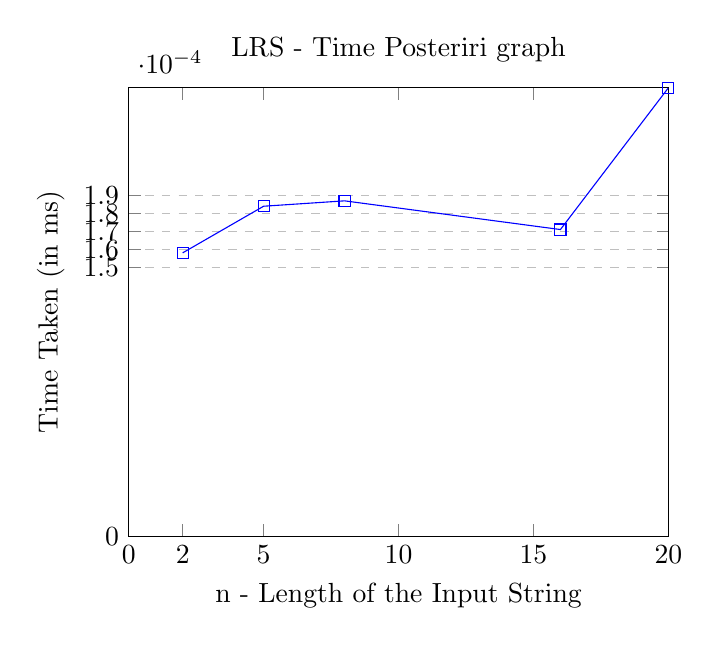
\begin{tikzpicture}
\begin{axis}[
    title={LRS - Time Posteriri graph},
    xlabel={n - Length of the Input String},
    ylabel={Time Taken (in ms)},
    xmin=0, xmax=20,
    ymin=0, ymax=0.00025,
    xtick={0,2,5,10,15,20},
    ytick={0,0.000150,0.000160,0.000170,0.000180,0.000190},
    legend pos=north west,
    ymajorgrids=true,
    grid style=dashed,
]

\addplot[
    color=blue,
    mark=square,
    ]
    coordinates {
    (2, 0.000158)(5,0.000184)(8,0.000187)(16,0.000171)(20,0.000250)
    };
    
\end{axis}
\end{tikzpicture}

\subsection{Space Complexity}
In the following table some cases are plotted
\begin{center}
 \begin{tabular}{||c | c | c||} 
 \hline
 Input & n & Space Occupied (in KB) \\ [0.5ex] 
 \hline\hline
 ab & 2 & 2776 \\ 
 \hline
 aabaa & 5 & 2904 \\
 \hline
 aaaaaaaaaa & 10 & 2812 \\
 \hline
 abaacddefrferghh & 16 & 2796 \\
 \hline
 aabaddefrghhuvdsused & 20 & 2912 \\ [1ex] 
 \hline
\end{tabular}
\end{center}

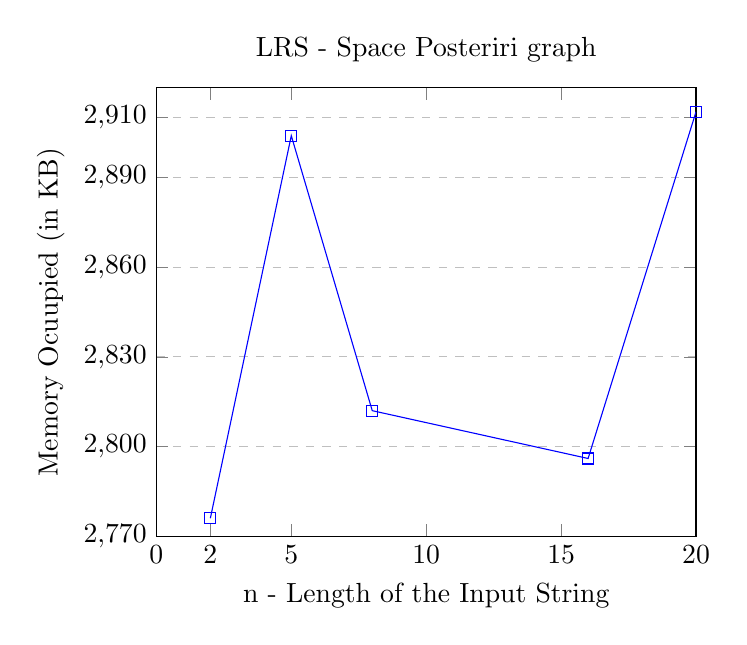
\begin{tikzpicture}
\begin{axis}[
    title={LRS - Space Posteriri graph},
    xlabel={n - Length of the Input String},
    ylabel={Memory Ocuupied (in KB)},
    xmin=0, xmax=20,
    ymin=2770, ymax=2920,
    xtick={0,2,5,10,15,20},
    ytick={2770,2800,2830,2860,2890,2910,2940},
    legend pos=north west,
    ymajorgrids=true,
    grid style=dashed,
]

\addplot[
    color=blue,
    mark=square,
    ]
    coordinates {
    (2, 2776)(5,2904)(8,2812)(16,2796)(20,2912)
    };
    
\end{axis}
\end{tikzpicture}

\section{Conclusion}
Using Dynamic Programming, we have reduced our time complexity to O(n$^{2}$) from the complexity of O(2$^{n}$) obtained by using brute force or naive solution from using recursion.

\section{Acknowledgment}
We are very much grateful to our Course instructor Mr.Rahul kala and our mentor, Mr.Md Meraz, who have provided the great opportunity to do this wonderful work on the subject of Data Structure and Algorithm Analysis specifically on methodologies of Dynamic Programming.

\section{References}

\begin{enumerate}
1.https://en.wikipedia.org/wiki/Dynamic-programming\newline
2.https://www.geeksforgeeks.org/printing-longest-common-subsequence/\newline
3.https://www.educative.io/courses/grokking-dynamic-programming-patterns-for-coding-interviews/m2G1pAq0OO0\newline
4.http://web.mit.edu/15.053/www/AMP-Chapter-11.pdf\newline
\end{enumerate}

\section{Appendix}

\subsection{Project link on Github:}
https://github.com/maggi2k19/DaaAssignments

\end{document}
